\section{Experiments}\label{sec:dttts.experiments}

\subsection{Some synthetic results}\label{sec:dttts.experiments.synthetic}
We first provide some synthetic experimental results comparing \DTTTS{} to \Hyperband{} and \ISHA{}. For these experiments, the arms are Bernoulli distributed and the reservoir distribution $\nu_0$ is fixed to some $\text{Beta}(a,b)$ distribution. 

\ISHA is the extension of \SHA to the \gls{siab} setting. It consists in running \SHA{} on a fixed number of arms drawn from the reservoir. Observe that for a total budget $B$, there exists a maximum number of arms $K^\star$ that can be processed by \SHA{}, which satisfies $B = \ceil{K^\star\log_2(K^\star)}$. Following~\cite{aziz2018infinite}, we run \ISHA with $K^\star$ arms drawn from the reservoir. % seems to be empirically performing better than \Hyperband.

We report in Fig.\,\ref{fig:dttts} the simple regret as a function of time for different algorithms and four Beta reservoir distributions. $\HTTTS$ and $\DTTTS$ are run with $\beta=1/2$ which is known to be a robust choice \citep{russo2016ttts}. Each point represents the expected simple regret $\mathbb{E}[1 - \mu_{I_n^*}]$ estimated over 1000 replications for an algorithm run with budget $n$. \DTTTS is very competitive on 3 reservoirs and \HTTTS is sometimes better, sometimes worse than \Hyperband. We also tried the \SiRI algorithm \citep{carpentier2015siri} (with $b$ as the tail parameter when $\nu_0=$Beta$(a,b)$) but obtained worse performance and therefore do not report the results.

\begin{figure}[ht]
  \centering
  \begin{subfigure}[t]{0.33\textwidth}
    \centering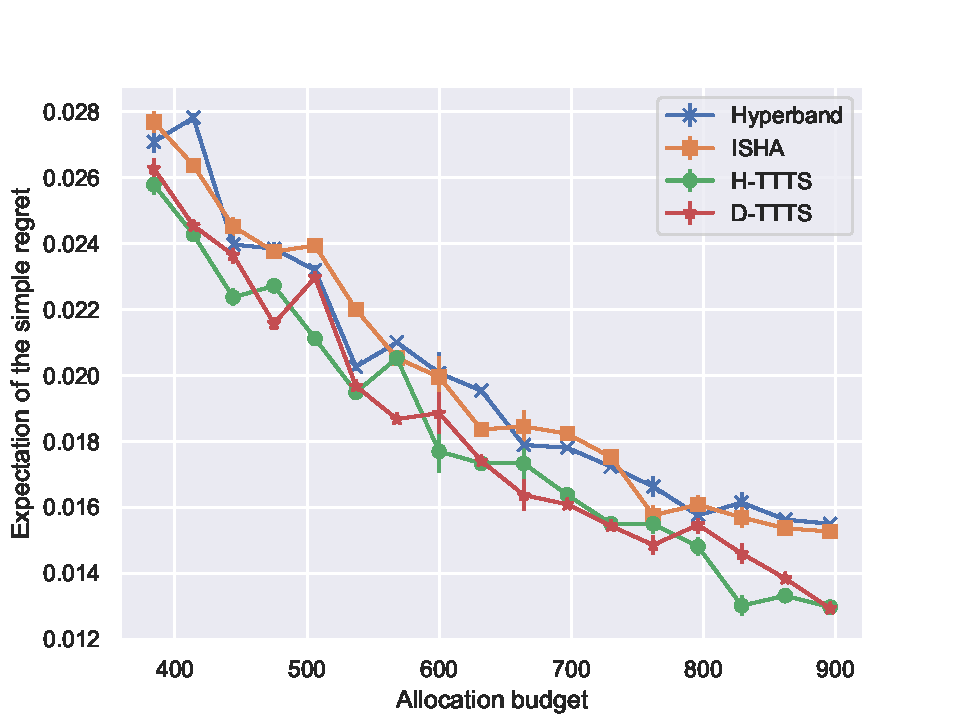
\includegraphics[width=\textwidth]{Chapter6/img/infinite/beta_1_1.pdf}
    \caption{Beta(1,1)}
  \end{subfigure}%
\begin{subfigure}[t]{0.33\textwidth}
    \centering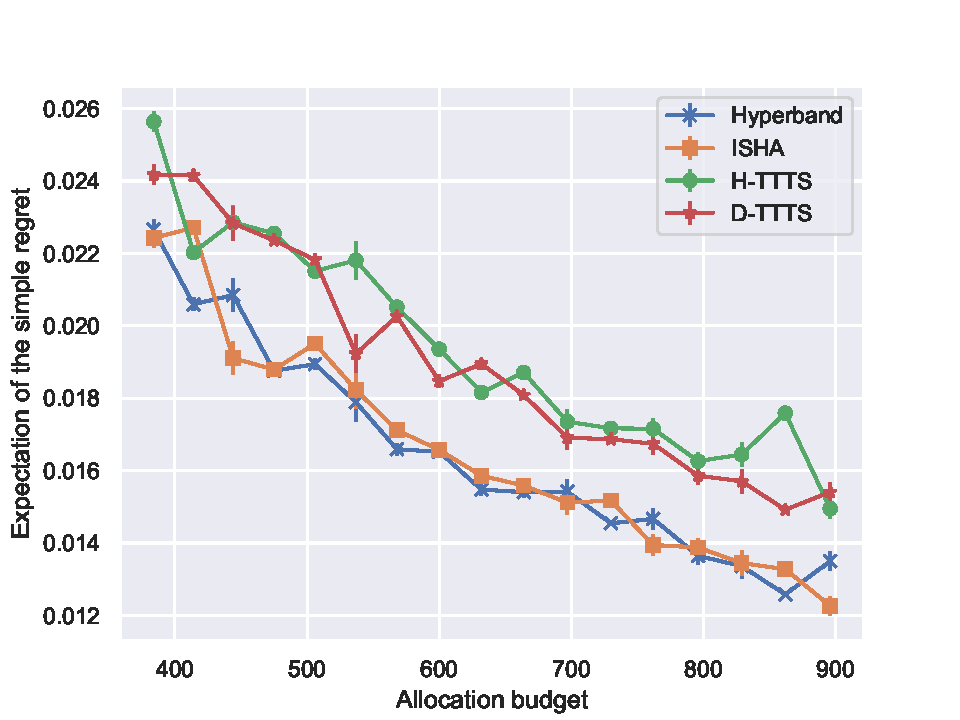
\includegraphics[width=\textwidth]{Chapter6/img/infinite/beta_3_1.pdf}
    \caption{Beta(3,1)}
  \end{subfigure}
  \begin{subfigure}[t]{0.33\textwidth}
    \centering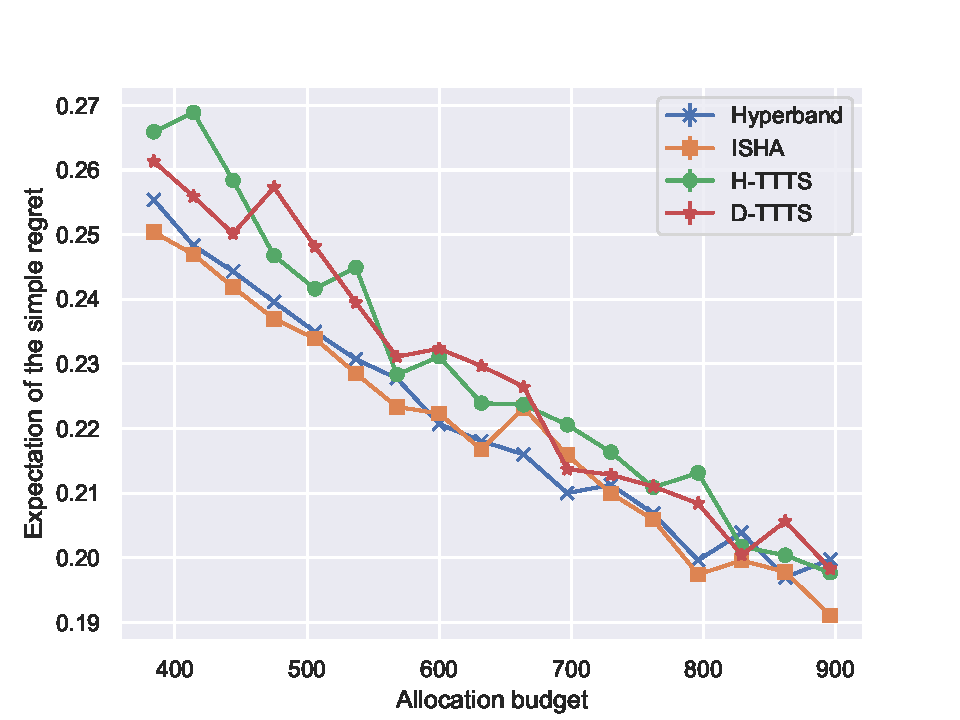
\includegraphics[width=\textwidth]{Chapter6/img/infinite/beta_1_3.pdf}
    \caption{Beta(1,3)}
  \end{subfigure}%
  \begin{subfigure}[t]{0.33\textwidth}
    \centering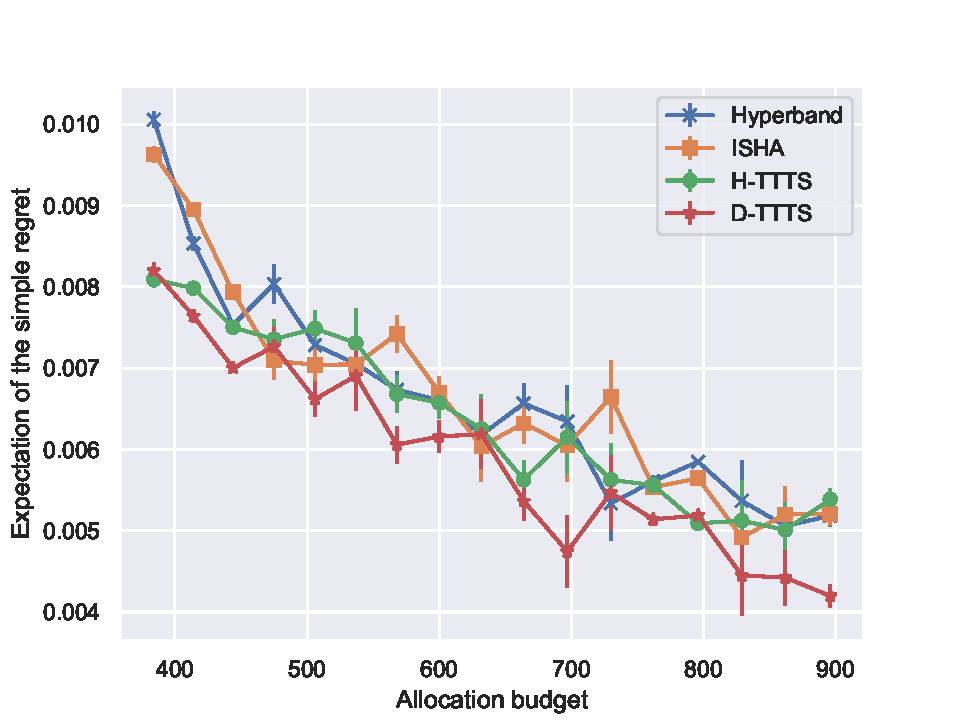
\includegraphics[width=\textwidth]{Chapter6/img/infinite/beta_-5_-5.pdf}
    \caption{Beta(0.5,0.5)}
  \end{subfigure}
  \caption{Simple regret of \DTTTS (against \Hyperband) as a function of the number of arms evaluations for different Beta reservoir.}
  \label{fig:dttts}
\end{figure}

Note that in the implementation of \Hyperband for this \emph{stochastic} infinite bandit setting, the elimination phase of the underlying \SHA algorithm is carried out according to the averaged loss of previous samples (as samples from an arm are i.i.d. in this setting and not a converging sequence). In the next section, we apply our algorithm to some real hyper-parameter optimization tasks. 

%\begin{figure}[ht]
%  \centering
%  \begin{subfigure}[t]{0.2\textwidth}
%    \centering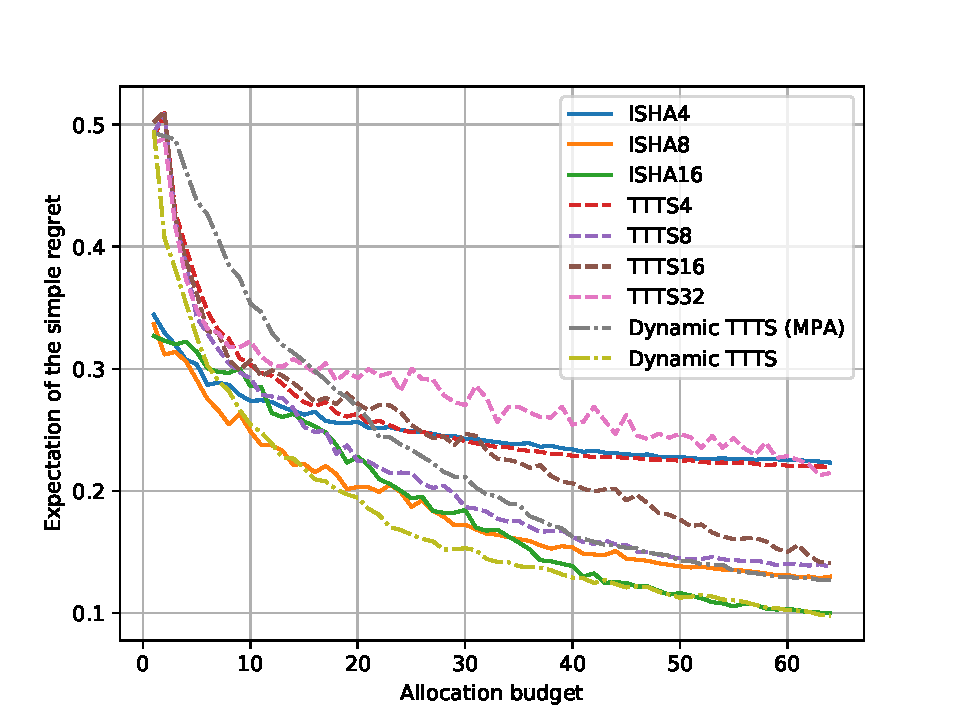
\includegraphics[width=\textwidth]{Chapter6/img/infinite/beta_1_1_64.pdf}
%    \caption{Beta(1,1)}
%  \end{subfigure}%
%  \begin{subfigure}[t]{0.2\textwidth}
%    \centering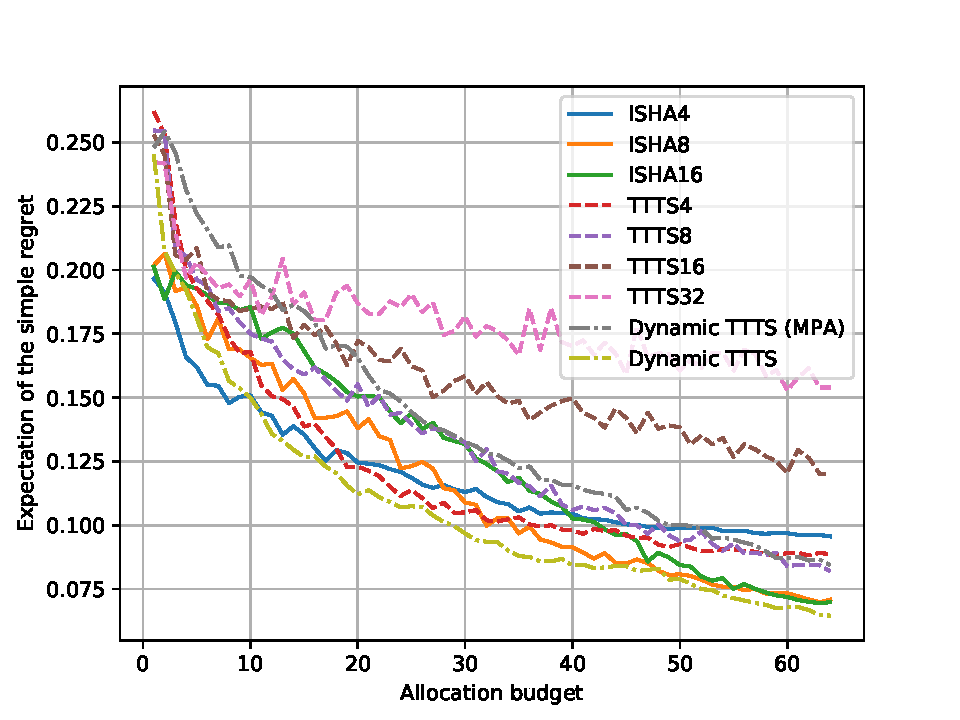
\includegraphics[width=\textwidth]{Chapter6/img/infinite/beta_3_1_64.pdf}
%    \caption{Beta(3,1)}
%  \end{subfigure}
%  \begin{subfigure}[t]{0.2\textwidth}
%    \centering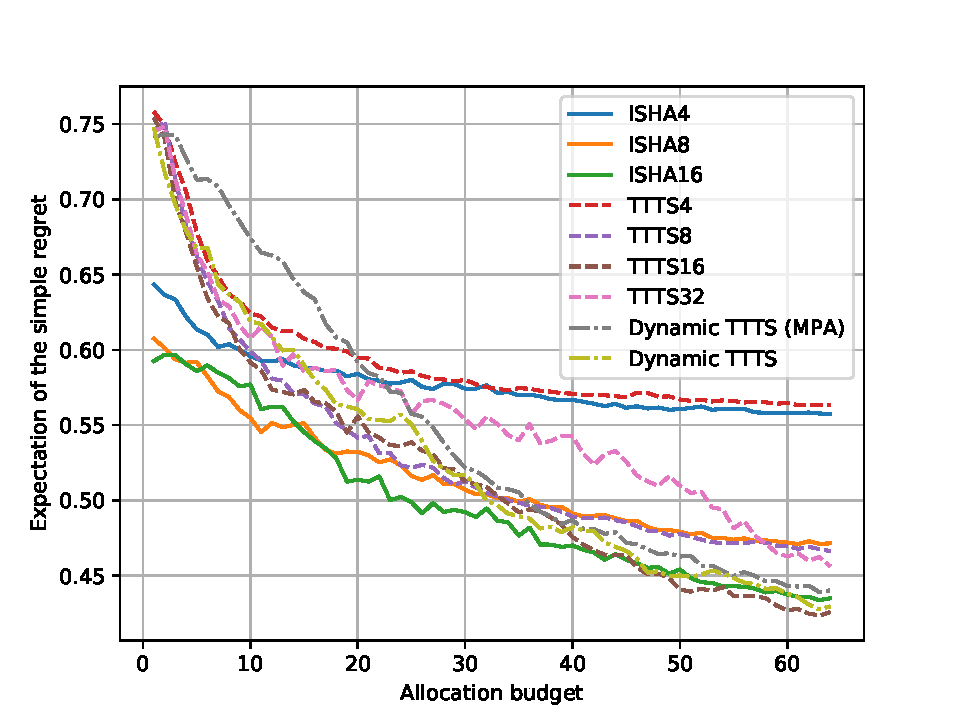
\includegraphics[width=\textwidth]{Chapter6/img/infinite/beta_1_3_64.pdf}
%    \caption{Beta(1,3)}
%  \end{subfigure}%
%  \begin{subfigure}[t]{0.2\textwidth}
%    \centering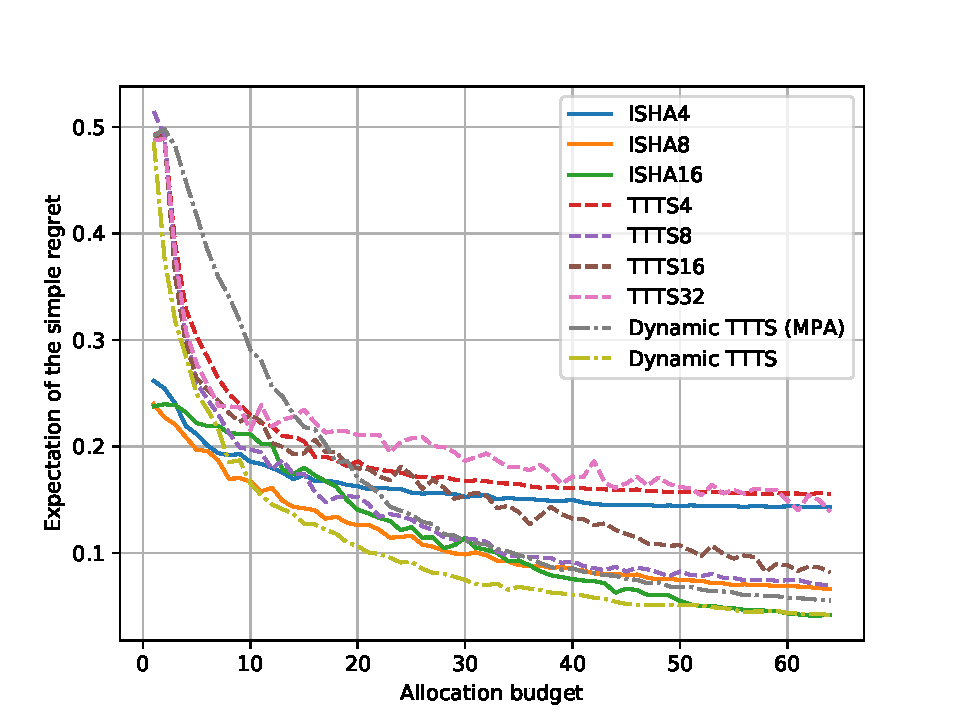
\includegraphics[width=\textwidth]{Chapter6/img/infinite/beta_-5_-5_64.pdf}
%    \caption{Beta(0.5,0.5)}
%  \end{subfigure}
%  %\begin{subfigure}[t]{0.2\textwidth}
%  %  \centering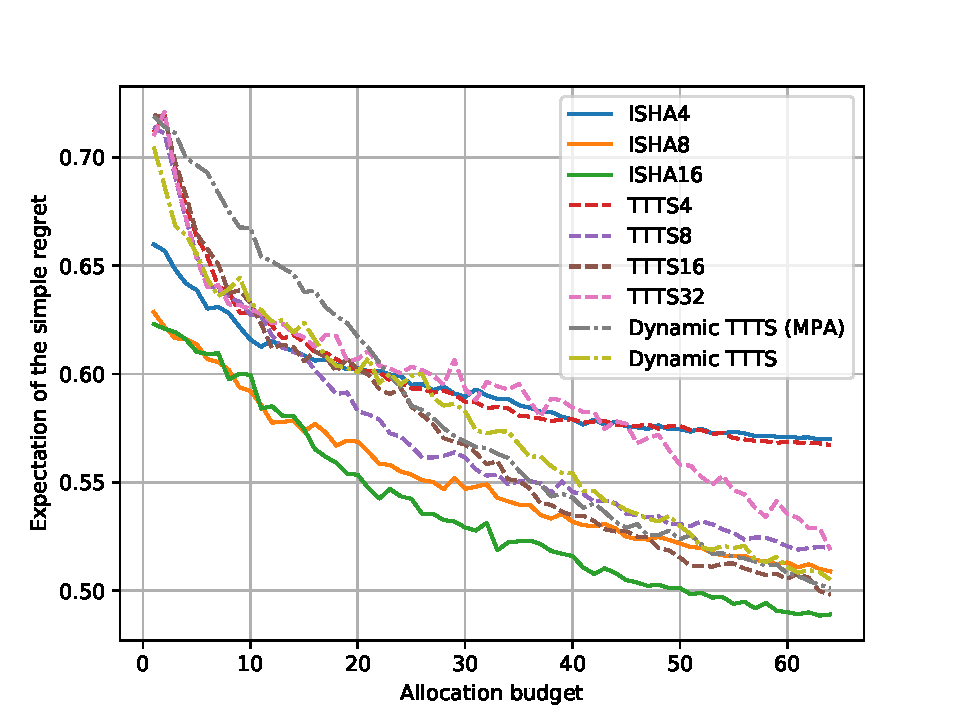
\includegraphics[width=\textwidth]{Chapter6/img/infinite/beta_2_5_64.pdf}
%  %  \caption{Beta(2,5)}
%  %\end{subfigure}
%  %\begin{subfigure}[t]{0.2\textwidth}
%  %  \centering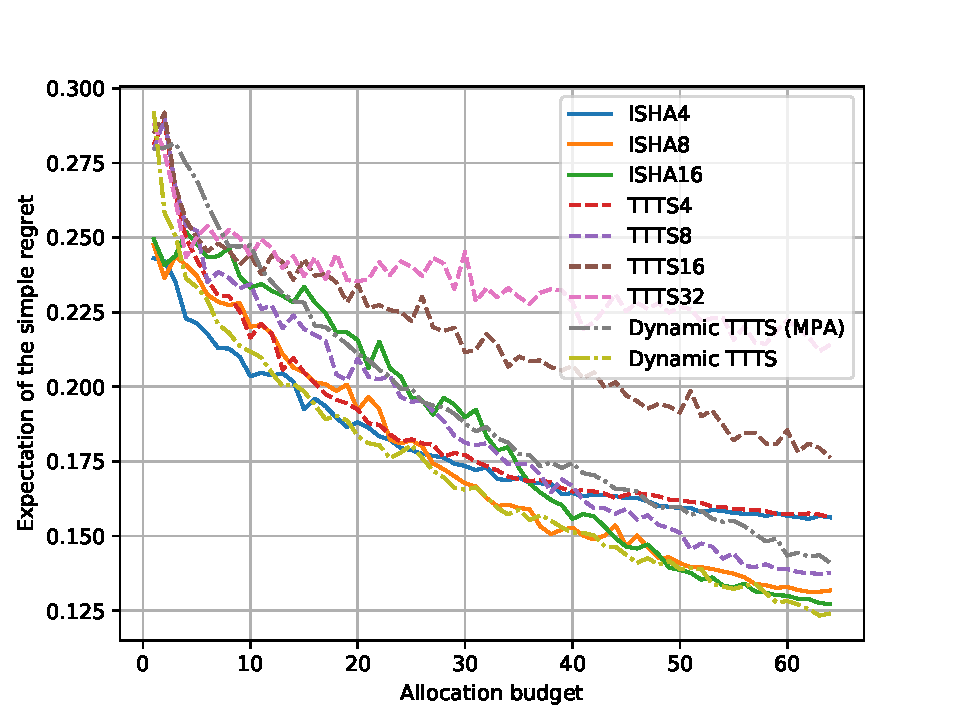
\includegraphics[width=\textwidth]{Chapter6/img/infinite/beta_5_2_64.pdf}
%  %  \caption{Beta(5,2)}
%  %\end{subfigure}
%  %\begin{subfigure}[t]{0.2\textwidth}
%  %  \centering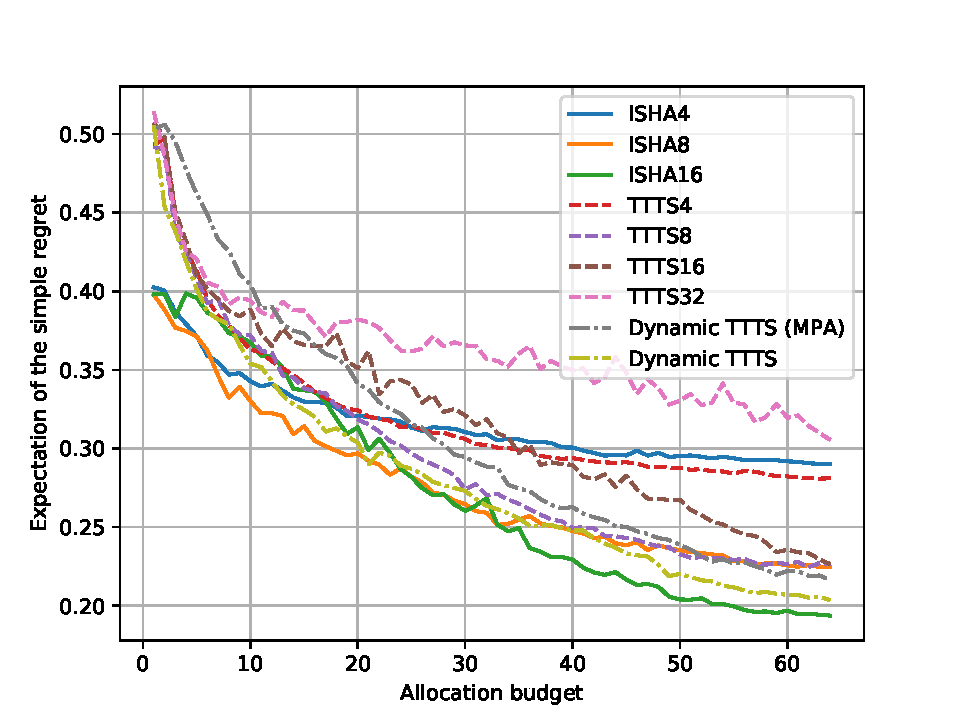
\includegraphics[width=\textwidth]{Chapter6/img/infinite/beta_2_2_64.pdf}
%  %  \caption{Beta(2,2)}
%  %\end{subfigure}
%  %\begin{subfigure}[t]{0.2\textwidth}
%  %  \centering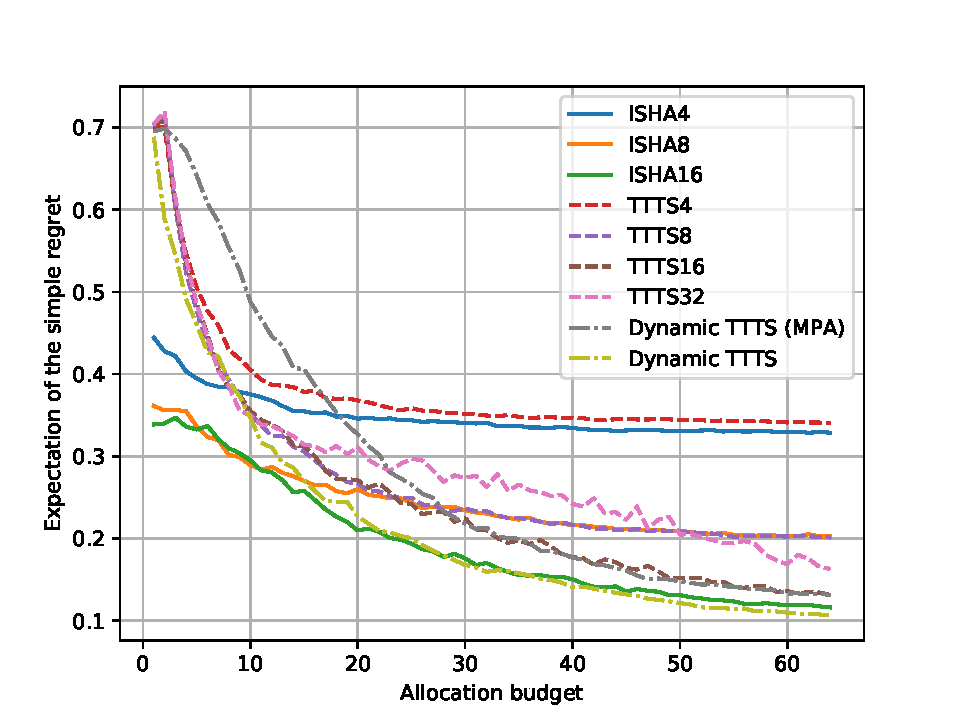
\includegraphics[width=\textwidth]{Chapter6/img/infinite/beta_-3_-7_64.pdf}
%  %  \caption{Beta(0.3,0.7)}
%  %\end{subfigure}
%  \caption{}
%  \label{fig:dttts1}
%\end{figure}

\subsection{Experiments on real datasets}\label{sec:dttts.experiments.real}
We now benchmark our bandit-based strategy against different types of HPO algorithms, namely, \TPE, random search, \Hyperband and \HTTTS{}, for the tuning of classifiers (\SVM and \MLP) on 4 different classification tasks: \textit{wine}, \textit{breast cancer}, and \textit{adult} datasets from \UCI machine learning repository \citep{dua2017}; and the \MNIST dataset~\citep{lecun1998gradient}.

For all the methods, a noisy evaluation of the black-box function $f$ (see the terminology introduced in Section~\ref{sec:dttts.framework}) for a hyper-parameter configuration $\bm\lambda$ consists in performing a shuffled 3-fold cross-validation on $\cD_{\texttt{train}}$. More precisely, given a random partitioning $\cup_{j=1}^3\cD_{\texttt{valid}}^j$ of $\cD_{\text{train}},$ where the folds are of equal size, we train a classifier $\hat{g}^{\,(j)}_{\bm\lambda}$ on $\cD_{\texttt{train}} \backslash \cD_{\texttt{valid}}^j$ for each fold $j$ and compute the average validation error defined as 
\[
    e \triangleq 1/|\cD_{\texttt{train}}|\sum_{j=1}^{3} \sum_{i \in \cD_{\text{valid}}^j} \mathbbm{1}\{\hat{g}^{\,(j)}_{\blambda}(\bx_i)\neq\by_i\}\,,
\]
which we report as a noisy estimate of the risk 
\[
    f(\bm\lambda) \triangleq \bP(\hat{g}^{\,(n)}_{\bm\lambda}(\bm X) \neq \bm Y),.
\]

Observe that both the noisy evaluation and the value of $f$ belong to $[0,1]$. Therefore we can introduce an \textit{arm} with rewards in $[0,1]$ for each hyper-parameter~$\bm\lambda$. Sampling  arm~$\bm\lambda$ produces reward $r \triangleq 1-e \in [0,1]$ with a different random partitioning and random seed for training for each selection. Arm~$\lambda$ is assumed to have mean of $1-f(\bm\lambda)$. In an infinite arm setting, querying a new arm from the reservoir corresponds to selecting a new hyper-parameter at random from the search space. With these two notions (\textit{arm sampling} and \textit{reservoir querying}), our algorithm for infinite BAI applies to HPO.  

For the experiments, we adapt the recommendation rule of \DTTTS to the HPO applications considered and always recommend the hyper-parameter configuration that has produced the smallest cross-validation error so far (which is also the recommendation rule used by other approaches, e.g., \Hyperband). For all methods, we report the cross-validation error for the recommended hyper-parameter configuration, as a function of time. We stress again that, unlike in standard bandits, where we could use the simple regret as a performance metric, we do not have access to the ground truth generalization error in real classification tasks. Therefore, we only report a proxy of the true error rate that we are interested in.

\paragraph{Results.} We first benchmark\footnote{Code at \url{http://researchers.lille.inria.fr/~valko/hp/publications/shang2019simple.code.zip}} our methods on a few simple \UCI datasets using \SVM from \Scikit as the classifier. We  optimize over two hyper-parameters: the \emph{penalty parameter} $C$ and the \emph{kernel coefficient}~$\gamma$\footnote{$\gamma$ is the parameter of the RBF kernel defined as $\exp(-\gamma||\bx-\bx'||^2)$}
for an RBF kernel, for which the pre-defined search bounds are both $\left[10^{-5}, 10^{5} \right]$.

%\begin{table}[ht]
%\centering
%\begin{tabular}{@{}l|lll@{}}
%\toprule
%\textbf{Classifier} & \textbf{Hyper-parameter}             & \textbf{Type}  & %\textbf{Bounds}                          \\ \midrule
%\Ada & \texttt{learning\_rate}      & $\mathbb{R}^+$ & $\left[10^{-5}, 10^{-1}\right]$                         \\
%& \texttt{n\_estimators}       & Integer        & $\left\lbrace 5,\dots, 200 \right\rbrace$ \\ \midrule
%& \texttt{learning\_rate}      & $\mathbb{R}^+$ & $\left[10^{-5}, 10^{-2}\right]$                         \\
%\GBM & \texttt{n\_estimators}       & Integer        & $\left\lbrace 10,\dots, 100 \right\rbrace$ \\
%& \texttt{max\_depth}          & Integer        & $\left\lbrace 2, \dots, 100 \right\rbrace$ \\
%& \texttt{min\_samples\_split}  & Integer        & $\left\lbrace 2, \dots, 100 \right\rbrace$ \\ \midrule
%\KNN & $k$                & Integer       & $\left\lbrace 10, \dots,50 \right\rbrace$ \\ \midrule
%\SVM & $C$                & $\mathbb{R}^+$ & $\left[ 10^{-5}, 10^{5} \right]$ \\
%& $\gamma$           & $\mathbb{R}^+$ & $\left[10^{-5}, 10^{5} \right]$  \\ \bottomrule
%\end{tabular}
%\caption{Hyper-parameters to be optimized for \UCI experiments.}
%\label{hyper_uci}
%\end{table}

%\todo{For the figures, can we have less white space and bigger figures? (probably some margin, or use crop)}
\begin{figure}[ht]
	\centering
	\begin{subfigure}[t]{0.33\textwidth}
    		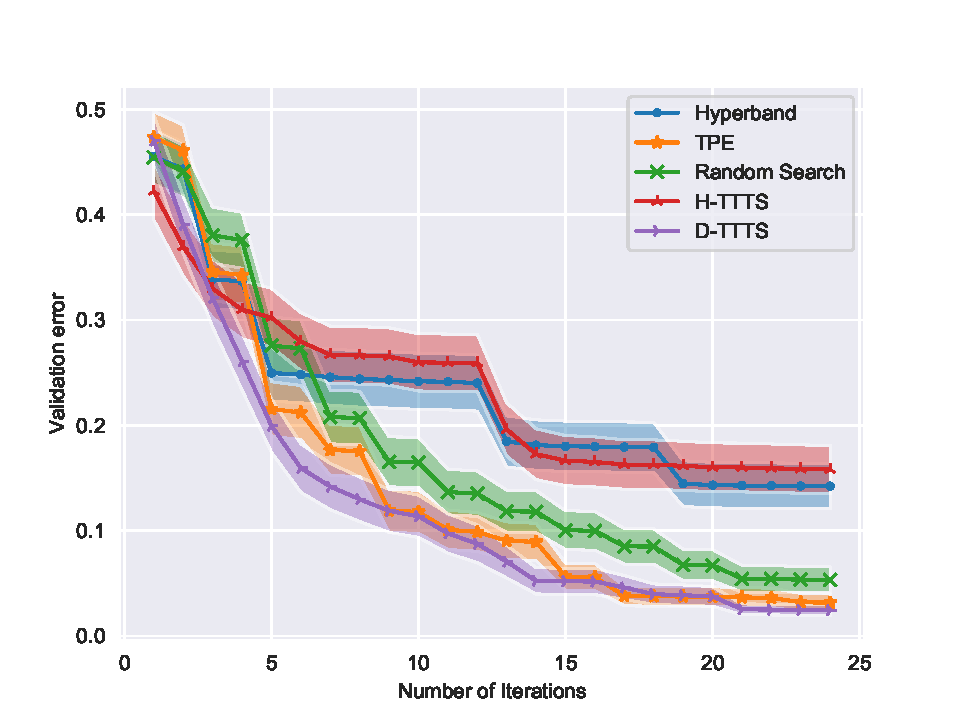
\includegraphics[width=\textwidth]{Chapter6/img/uci/wine.pdf}
    		\caption{wine}
    		\label{fig:wine}
	\end{subfigure}
	\begin{subfigure}[t]{0.33\textwidth}
    		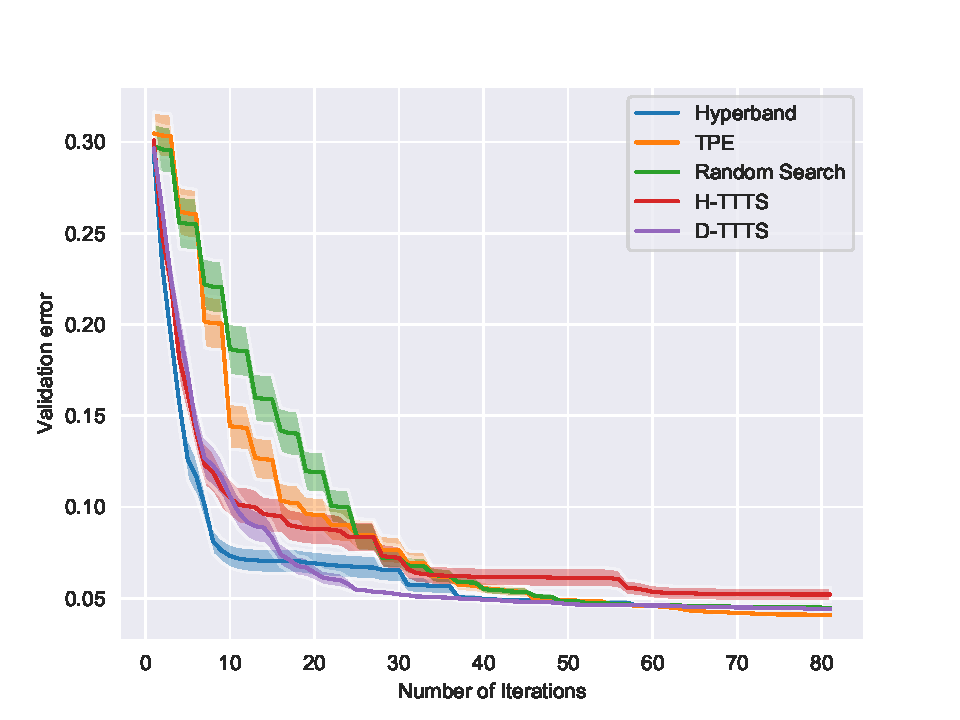
\includegraphics[width=\textwidth]{Chapter6/img/uci/breast_cancer.pdf}
    		\caption{breast cancer}
    		\label{fig:breast_cancer}
	\end{subfigure}
	\begin{subfigure}[t]{0.33\textwidth}
    		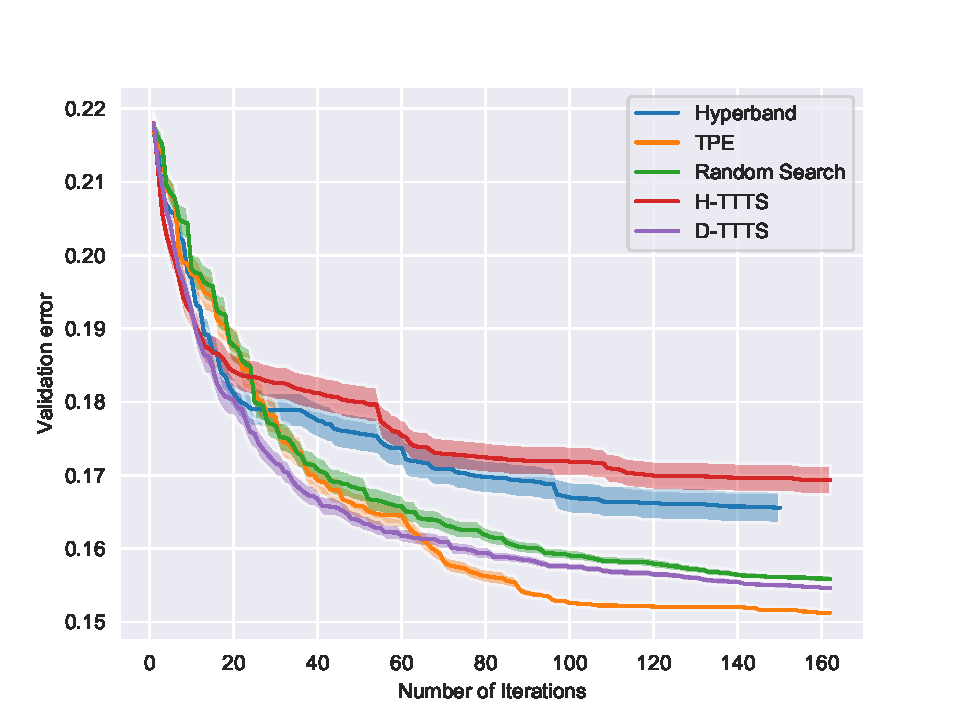
\includegraphics[width=\textwidth]{Chapter6/img/uci/adult.pdf}
    		\caption{adult}
    		\label{fig:adult}
	\end{subfigure}
	\begin{subfigure}[t]{0.33\textwidth}
    		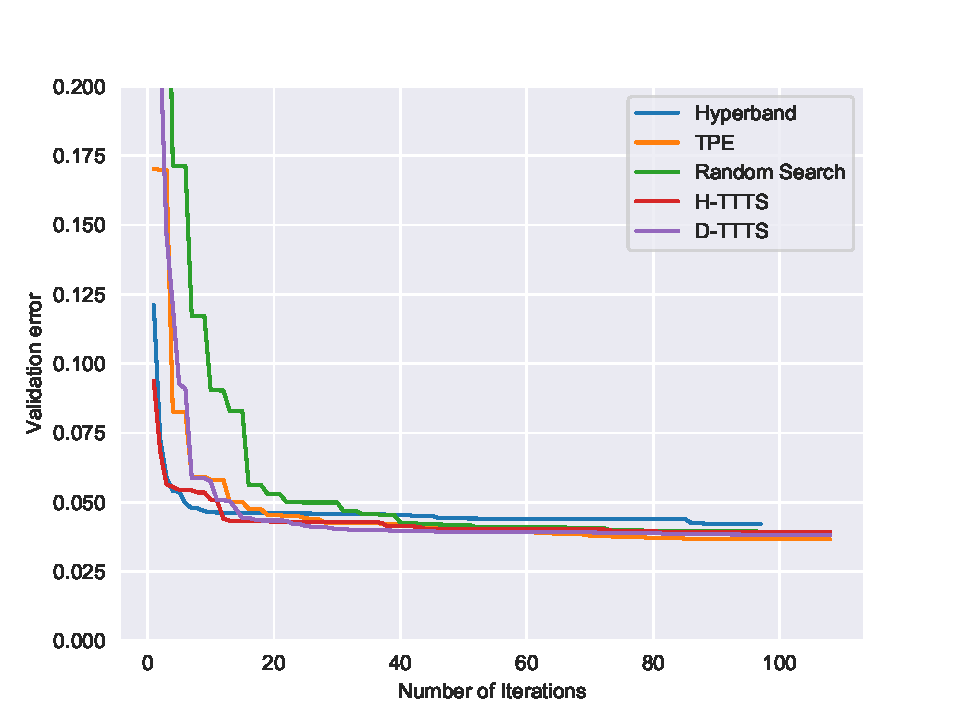
\includegraphics[width=\textwidth]{Chapter6/img/mnist/mnist.pdf}
    		\caption{\MNIST}
    		\label{fig:mnist}
	\end{subfigure}
	\caption{Mean cross-validation error of different HPO algorithms with (a) \SVM run on the \UCI wine dataset, (b) \SVM run on the \UCI breast cancer dataset, (c) \SVM run on the \UCI adult dataset and (d) \MLP run on the \MNIST dataset.}
\end{figure}

Fig.\,\ref{fig:wine} shows the mean cross-validation error of \SVM run on the \UCI wine dataset over 24 pulls\footnote{The number of pulls here and later is chosen exactly as in the work of \citet{li2017hyperband}} averaged on 100 runs. The task is to predict the quality score  of wine (between 0 and 10) given 11 attributes. Recall that one iteration corresponds to one arm pull. In this experiment, \DTTTS improves over other benchmark algorithms. Fig.\,\ref{fig:breast_cancer} is the same experiment run on the \UCI breast cancer dataset over 81 pulls. The task is to predict whether a patient has breast cancer based on 32 attributes. We repeat the experiment 100 times. This time, \DTTTS is slightly worse than \Hyperband at the beginning, but improves later. Finally, we optimize \SVM on a relatively more complicated \UCI adult dataset over 162 pulls, for which the result is shown in Fig.\,\ref{fig:adult}. The task is to tell whether the income of an individual is higher than 50k or not given 14 attributes. This experiment is also averaged over 100 runs. \DTTTS is better than other algorithms at the beginning, but is outperformed by \TPE towards the end. We see that, although not always the best, \DTTTS shows a consistent, robust, and quite competitive performance in the 3 tasks. 

We now carry out the classic \MNIST digits classification task using multi-layer perceptron (\MLP). We choose to optimize over three hyper-parameters: the \emph{size of hidden layer} (an integer between 5 and 50), the \emph{$\ell_2$ penalty parameter} $\alpha$ (between 0 and 0.9) and the \emph{initial learning rate} (bounded in $\left[10^{-5}, 10^{-1} \right]$). Fig.\,\ref{fig:mnist} shows the result of \MLP run on \MNIST over 108 pulls, this time averaged over 20 runs. \DTTTS is slightly worse than \Hyperband and \HTTTS in the very beginning, but is performing well afterward. %We notice that, although always showing bad performance in the \UCI tasks, \HTTTS shows a good behavior for the \MNIST task.

%\begin{table}[ht]
%\centering
%\begin{tabular}{@{}l|lll@{}}
%\toprule
%\textbf{Classifier} & \textbf{Hyper-parameter}             & \textbf{Type}  & \textbf{Bounds}                          \\ \midrule
%\MLP & \texttt{hidden\_layer\_size} & Integer          & $\left[5, 50\right]$  \\
%& \texttt{alpha}               & $\mathbb{R}^{+}$ & $\left[0, 0.9\right]$ \\ 
%& \texttt{learning\_rate\_init} & $\mathbb{R}^{+}$ & $\left[ 10^{-5}, 10^{-1} \right]$ \\ \bottomrule
%\end{tabular}
%\caption{Hyper-parameters to be optimized for \MNIST experiments.}
%\label{hyper_mnist}
%\end{table}

% \begin{figure}[ht]
%     \centering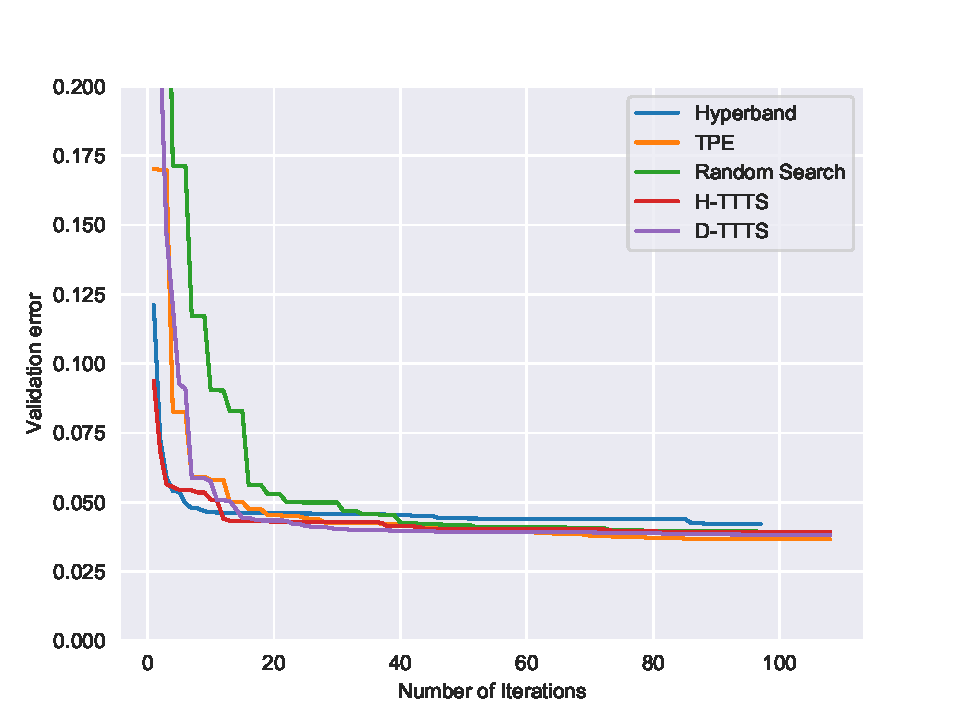
\includegraphics[width=0.6\textwidth]{Chapter6/img/mnist/mnist.pdf}
%     \caption{\MNIST dataset}
%     \label{fig:mnist}
% \end{figure}
